\documentclass[svgnames,11pt]{beamer}
\setbeamercolor{structure}{fg=SlateGray}
\usetheme{Goettingen}
\input{/home/tof/Documents/Cozy/latex-include/preambule_commun.tex}
%\usepackage{pgfpages}
%\setbeameroption{show notes on second screen=left}
\author[]{Christophe Viroulaud}
\title{Chiffrement asymétrique\\Diffie-Hellman}
\date{}
%\logo{}
%\institute{Seconde SNT}
%\institute{Première NSI}
\institute{Terminale NSI}
\setbeamertemplate{navigation symbols}{}
\setbeamertemplate{footline}[frame number]
\usepackage{tikz}

\begin{document}
\begin{frame}
    \titlepage
\end{frame}

\section{Problématique}
\begin{frame}
    \frametitle{Problématique}
    Le chiffrement symétrique est très efficace mais il souffre d'un défaut majeur: il faut que la source et le destinataire utilise la même clé de chiffrement.
    \begin{center}
        \centering
        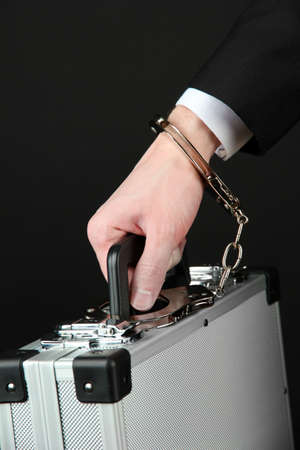
\includegraphics[width=3cm]{ressources/echange.jpg}
    \end{center}
    \begin{center}
        \framebox{Peut-on échanger une clé de manière sécurisée?}
    \end{center}
\end{frame}

\section{S'aider des mathématiques}
\subsection{Principe}
\begin{frame}
    \frametitle{Les mathématiques à la rescousse}
    \begin{itemize}
        \item<1-> 1974: Le puzzle de Merkle s'appuie sur le coût long du décryptage.
        \item<2-> 1976: \textbf{Diffie et Hellman} utilise une fonction mathématique avec des propriétés particulières
    \end{itemize}


\end{frame}

\begin{frame}
    \frametitle{Propriétés}

    \begin{itemize}
        \item<1-> La fonction $f$ est connue de tous.
        \item<2-> Si on connaît $f(x,y)$ et $x$ alors il est difficile de retrouver $y$.
        \item<3-> Pour tous entiers $x,y,z$, $$f(f(x,y),z)=f(f(x,z),y)$$
    \end{itemize}

\end{frame}
\begin{frame}
    \frametitle{}

    En pratique la fonction mathématique utilisée utilise les puissances et le modulo.

\end{frame}
\subsection{Analogie des couleurs}
\begin{frame}
    \frametitle{Analogie des couleurs}
\begin{center}
    \begin{tikzpicture}[scale=0.7]
        \node at(-6,0){Alice};
        \node at(0,0){Canal non sécurisé};
        \node at(6,0){Bob};
        \draw[dashed] (-3,0) -- (-3,-11) ;
        \draw[dashed] (3,0) -- (3,-11) ;

        \node[draw] at(0,-1){Étape 1};
        \node[fill=yellow] at(0,-2){x};
    \end{tikzpicture}
\end{center}
\note[item]{Si on connaît jaune et vert il est difficile de retrouver le bleu qui a été utilisé.}
    \note[item]{jaune et la fonction f sont connus de tous. En pratique jaune est un nombre premier (modulo) et f un nombre inférieur (base de la puissance)
        \begin{itemize}
            \item p = 23
            \item f = 5
        \end{itemize}}
\end{frame}

\begin{frame}
    \frametitle{Analogie des couleurs}
\begin{center}
    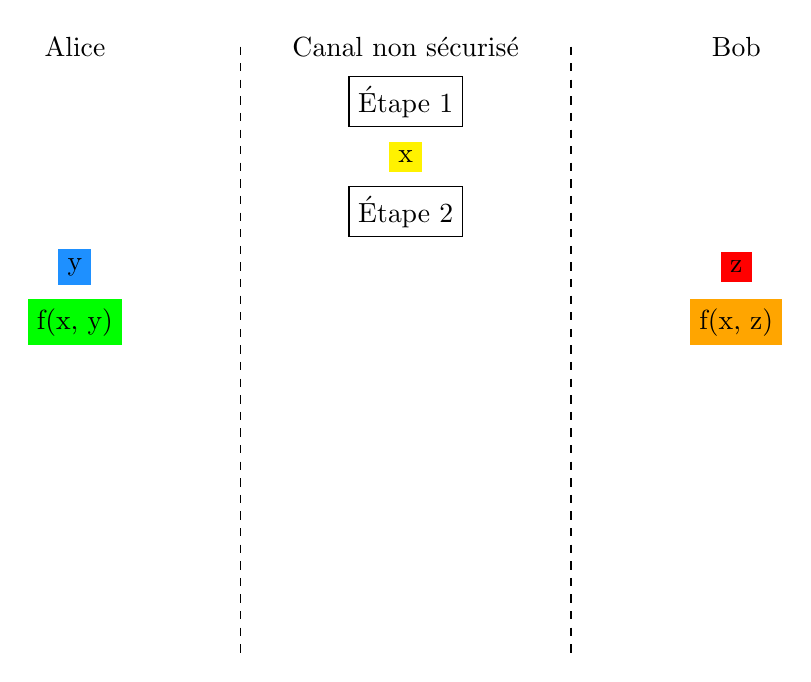
\begin{tikzpicture}[scale=0.7]
        \node at(-6,0){Alice};
        \node at(0,0){Canal non sécurisé};
        \node at(6,0){Bob};
        \draw[dashed] (-3,0) -- (-3,-11) ;
        \draw[dashed] (3,0) -- (3,-11) ;

        \node[draw] at(0,-1){Étape 1};
        \node[fill=yellow] at(0,-2){x};

        \node[draw] at(0,-3){Étape 2};
        \node[fill=DodgerBlue] at(-6,-4){y};
        \node[fill=Red] at(6,-4){z};
        \node[fill=Lime] at(-6,-5){f(x, y)};
        \node[fill=Orange] at(6,-5){f(x, z)};


    \end{tikzpicture}
\end{center}
    \note{y et z deux nombres: $f^y[mod x]$
    \begin{itemize}
        \item Alice: y = 6 $\rightarrow$ $5^6[23]=8$
        \item Bob: z = 15 $\rightarrow$ $5^{15}[23]=19$
    \end{itemize}}
\end{frame}

\begin{frame}
    \frametitle{Analogie des couleurs}

    \begin{center}
        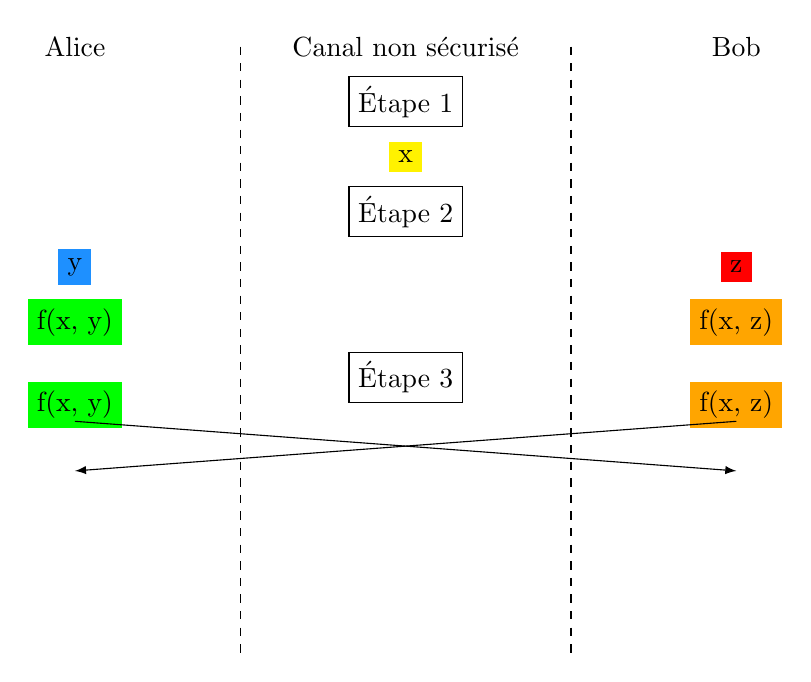
\begin{tikzpicture}[scale=0.7]
            \node at(-6,0){Alice};
            \node at(0,0){Canal non sécurisé};
            \node at(6,0){Bob};
            \draw[dashed] (-3,0) -- (-3,-11) ;
            \draw[dashed] (3,0) -- (3,-11) ;
    
            \node[draw] at(0,-1){Étape 1};
            \node[fill=yellow] at(0,-2){x};
    
            \node[draw] at(0,-3){Étape 2};
            \node[fill=DodgerBlue] at(-6,-4){y};
            \node[fill=Red] at(6,-4){z};
            \node[fill=Lime] at(-6,-5){f(x, y)};
            \node[fill=Orange] at(6,-5){f(x, z)};
    
            \node[draw] at(0,-6){Étape 3};
            \node[fill=Lime] at(-6,-6.5){f(x, y)};
            \node[fill=Orange] at(6,-6.5){f(x, z)};
            \draw[->,>=latex] (-6,-6.8) -- (6,-7.7);
            \draw[->,>=latex] (6,-6.8) -- (-6,-7.7);
    
        \end{tikzpicture}
    \end{center}
    \note{\begin{itemize}
            \item Alice envoie 8
            \item Bob envoie 19
        \end{itemize}}
\end{frame}

\begin{frame}
    \frametitle{Analogie des couleurs}

    \begin{center}
        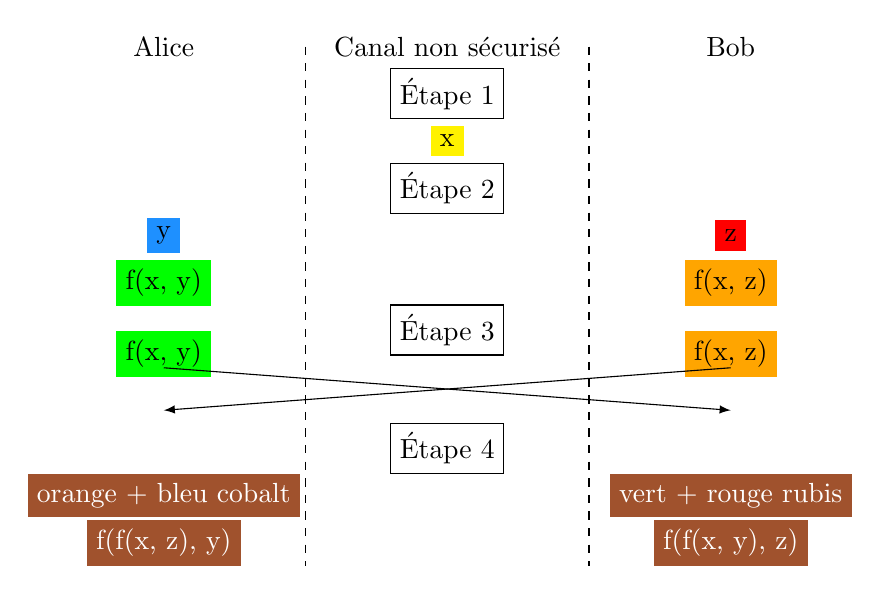
\begin{tikzpicture}[scale=0.6]
            \node at(-6,0){Alice};
            \node at(0,0){Canal non sécurisé};
            \node at(6,0){Bob};
            \draw[dashed] (-3,0) -- (-3,-11) ;
            \draw[dashed] (3,0) -- (3,-11) ;
    
            \node[draw] at(0,-1){Étape 1};
            \node[fill=yellow] at(0,-2){x};
    
            \node[draw] at(0,-3){Étape 2};
            \node[fill=DodgerBlue] at(-6,-4){y};
            \node[fill=Red] at(6,-4){z};
            \node[fill=Lime] at(-6,-5){f(x, y)};
            \node[fill=Orange] at(6,-5){f(x, z)};
    
            \node[draw] at(0,-6){Étape 3};
            \node[fill=Lime] at(-6,-6.5){f(x, y)};
            \node[fill=Orange] at(6,-6.5){f(x, z)};
            \draw[->,>=latex] (-6,-6.8) -- (6,-7.7);
            \draw[->,>=latex] (6,-6.8) -- (-6,-7.7);
    
            \node[draw] at(0,-8.5){Étape 4};
            \node[fill=Sienna,text=white] at(-6,-9.5){orange + bleu cobalt};
            \node[fill=Sienna,text=white] at(-6,-10.5){f(f(x, z), y)};
            \node[fill=Sienna,text=white] at(6,-9.5){vert + rouge rubis};
            \node[fill=Sienna,text=white] at(6,-10.5){f(f(x, y), z)};
    
        \end{tikzpicture}
    \end{center}
    \note[item]{Alice et Bob utilisent le marron comme clé de chiffrement}
    \note[item]{\begin{itemize}
            \item Alice: $19^6[23]=2$
            \item Bob: $8^{15}[23]=2$
        \end{itemize}}
    \note[item]{Il faut prendre plus grands nombres pour que brute force ne fonctionne pas.}
\end{frame}
\section{Faiblesse du protocole}
\begin{frame}
    \frametitle{Faiblesse}

    Il est mathématiquement très difficile pour Eve (\emph{eavesdropper: écouteuse}) de retrouver les valeurs choisies par Alice et Bob. Cependant, elle n'est pas obligée de le faire.

\end{frame}
\begin{frame}
    \frametitle{Man in the middle attack}

\begin{center}
    
    \begin{center}
        \begin{tikzpicture}[scale=0.7]
            \node at(-6,0){Alice};
            \node at(0,0){Canal non sécurisé};
            \node at(6,0){Bob};
            \draw[dashed] (-3,0) -- (-3,-11.5) ;
            \draw[dashed] (3,0) -- (3,-11.5) ;
    
            \node[draw] at(0,-1){Étape 1};
            \node[fill=yellow] at(0,-2){x};
    
    
        \end{tikzpicture}
    \end{center}
\end{center}

\end{frame}
\begin{frame}
    \frametitle{Man in the middle attack}

    \begin{center}
        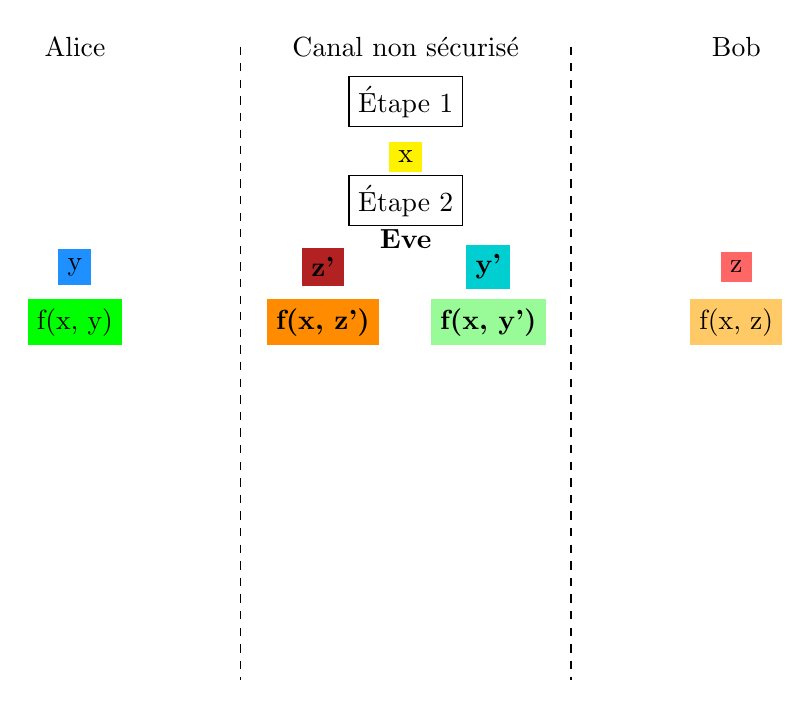
\begin{tikzpicture}[scale=0.7]
            \node at(-6,0){Alice};
            \node at(0,0){Canal non sécurisé};
            \node at(6,0){Bob};
            \draw[dashed] (-3,0) -- (-3,-11.5) ;
            \draw[dashed] (3,0) -- (3,-11.5) ;

            \node[draw] at(0,-1){Étape 1};
            \node[fill=yellow] at(0,-2){x};

            \node[draw] at(0,-2.8){Étape 2};
            \node at(0,-3.5){\textbf{Eve}};
            \node[fill=DarkTurquoise] at(1.5,-4){\textbf{y'}};
            \node[fill=PaleGreen] at(1.5,-5){\textbf{f(x, y')}};
            \node[fill=FireBrick] at(-1.5,-4){\textbf{z'}};
            \node[fill=DarkOrange] at(-1.5,-5){\textbf{f(x, z')}};
            \node[fill=DodgerBlue] at(-6,-4){y};
            \node[fill=Red!60] at(6,-4){z};
            \node[fill=Lime] at(-6,-5){f(x, y)};
            \node[fill=Orange!60] at(6,-5){f(x, z)};


        \end{tikzpicture}
        \captionof{figure}{Attaque de l'homme du milieu}
    \end{center}

\end{frame}


\begin{frame}
    \frametitle{Man in the middle attack}

    \begin{center}
        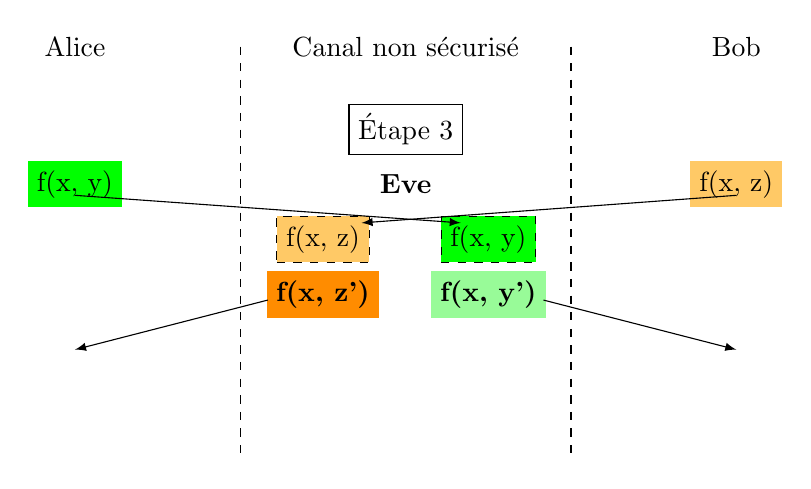
\begin{tikzpicture}[scale=0.7]
            \node at(-6,-4){Alice};
            \node at(0,-4){Canal non sécurisé};
            \node at(6,-4){Bob};
            \draw[dashed] (-3,-4) -- (-3,-11.5) ;
            \draw[dashed] (3,-4) -- (3,-11.5) ;

            \node[draw] at(0,-5.5){Étape 3};
            \node at(0,-6.5){\textbf{Eve}};
            \node[fill=PaleGreen] at(1.5,-8.5){\textbf{f(x, y')}};
            \node[fill=DarkOrange] at(-1.5,-8.5){\textbf{f(x, z')}};
            \node[fill=Lime,draw, dashed] at(1.5,-7.5){f(x, y)};
            \node[draw, dashed, fill=Orange!60] at(-1.5,-7.5){f(x, z)};
            \node[fill=Lime] at(-6,-6.5){f(x, y)};
            \node[fill=Orange!60] at(6,-6.5){f(x, z)};
            \draw[->,>=latex] (-6,-6.7) -- (1,-7.2);
            \draw[->,>=latex] (6,-6.7) -- (-0.8,-7.2);
            \draw[->,>=latex] (2.5,-8.6) -- (6,-9.5);
            \draw[->,>=latex] (-2.5,-8.6) -- (-6,-9.5);

        \end{tikzpicture}
    \end{center}

\end{frame}
\begin{frame}
    \frametitle{Man in the middle attack}

    \begin{center}
        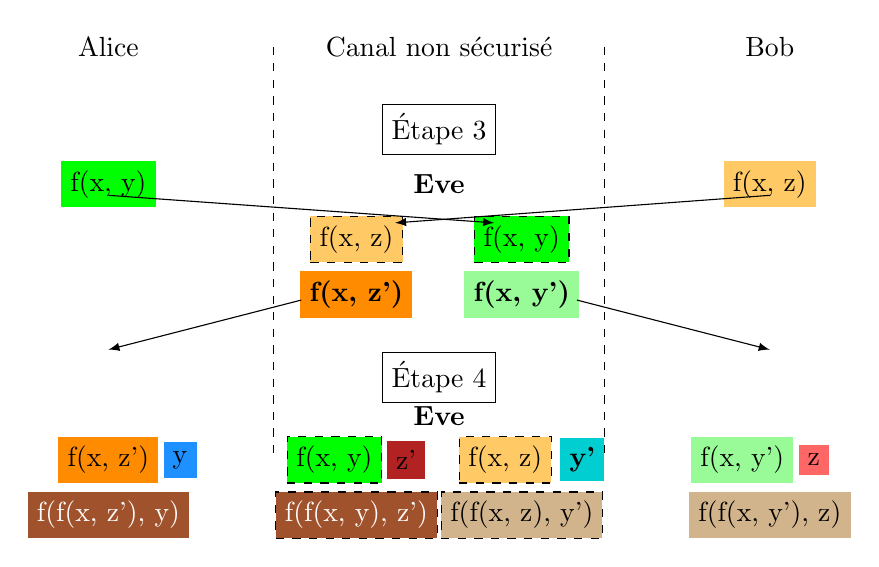
\begin{tikzpicture}[scale=0.7]
            \node at(-6,-4){Alice};
            \node at(0,-4){Canal non sécurisé};
            \node at(6,-4){Bob};
            \draw[dashed] (-3,-4) -- (-3,-11.5) ;
            \draw[dashed] (3,-4) -- (3,-11.5) ;

            \node[draw] at(0,-5.5){Étape 3};
            \node at(0,-6.5){\textbf{Eve}};
            \node[fill=PaleGreen] at(1.5,-8.5){\textbf{f(x, y')}};
            \node[fill=DarkOrange] at(-1.5,-8.5){\textbf{f(x, z')}};
            \node[fill=Lime,draw, dashed] at(1.5,-7.5){f(x, y)};
            \node[draw, dashed, fill=Orange!60] at(-1.5,-7.5){f(x, z)};
            \node[fill=Lime] at(-6,-6.5){f(x, y)};
            \node[fill=Orange!60] at(6,-6.5){f(x, z)};
            \draw[->,>=latex] (-6,-6.7) -- (1,-7.2);
            \draw[->,>=latex] (6,-6.7) -- (-0.8,-7.2);
            \draw[->,>=latex] (2.5,-8.6) -- (6,-9.5);
            \draw[->,>=latex] (-2.5,-8.6) -- (-6,-9.5);

            \node[draw] at(0,-10){Étape 4};
            \node at(0,-10.7){\textbf{Eve}};
            \node[fill=Lime,draw, dashed] at(-1.9,-11.5){f(x, y)};
            \node[fill=FireBrick] at(-0.6,-11.5){z'};
            \node[draw, dashed,fill=Sienna,text=white] at(-1.5,-12.5){f(f(x, y), z')};
            \node[draw, dashed,fill=Tan] at(1.5,-12.5){f(f(x, z), y')};
            \node[fill=DarkOrange] at(-6,-11.5){f(x, z')};
            \node[fill=DodgerBlue] at(-4.7,-11.5){y};

            \node[fill=Sienna,text=white] at(-6,-12.5){f(f(x, z'), y)};
            \node[draw, dashed, fill=Orange!60] at(1.2,-11.5){f(x, z)};
            \node[fill=DarkTurquoise] at(2.6,-11.5){\textbf{y'}};
            \node[fill=Tan] at(6,-12.5){f(f(x, y'), z)};
            \node[fill=PaleGreen] at(5.5,-11.5){f(x, y')};
            \node[fill=Red!60] at(6.8,-11.5){z};

        \end{tikzpicture}
    \end{center}

\end{frame}
\begin{frame}
    \frametitle{}

    \begin{aretenir}[]
        Le protocole de Diffie-Hellman permet d'échanger des clés par un canal non sécurisé. Cependant il n'assure pas l'\emph{authentification} des participants.
    \end{aretenir}

\end{frame}

\end{document}